\documentclass[pdftex]{article}
\usepackage[T1]{fontenc}
\usepackage[utf8]{inputenc}
\usepackage{graphicx}
\usepackage{caption}
\usepackage{titling}
\usepackage{enumitem}
\setlist[itemize]{leftmargin=*}
\setlist[description]{leftmargin=*}

\setlength{\droptitle}{-15em}
\title{PHYS 721 Homework 5}
\author{Nick Tyler}
\date{}


\begin{document}
\maketitle
\begin{enumerate}
	\item Three Breit-Wigner curves for the decay $\phi \rightarrow K^{+} K^{- }$ are fitted to data set 1. 
		The first fit, in green, is the relatavistic Breit-wigner. The second fit, in red, is the Non-Relatavistic
		Breit-Wigner curve. \

		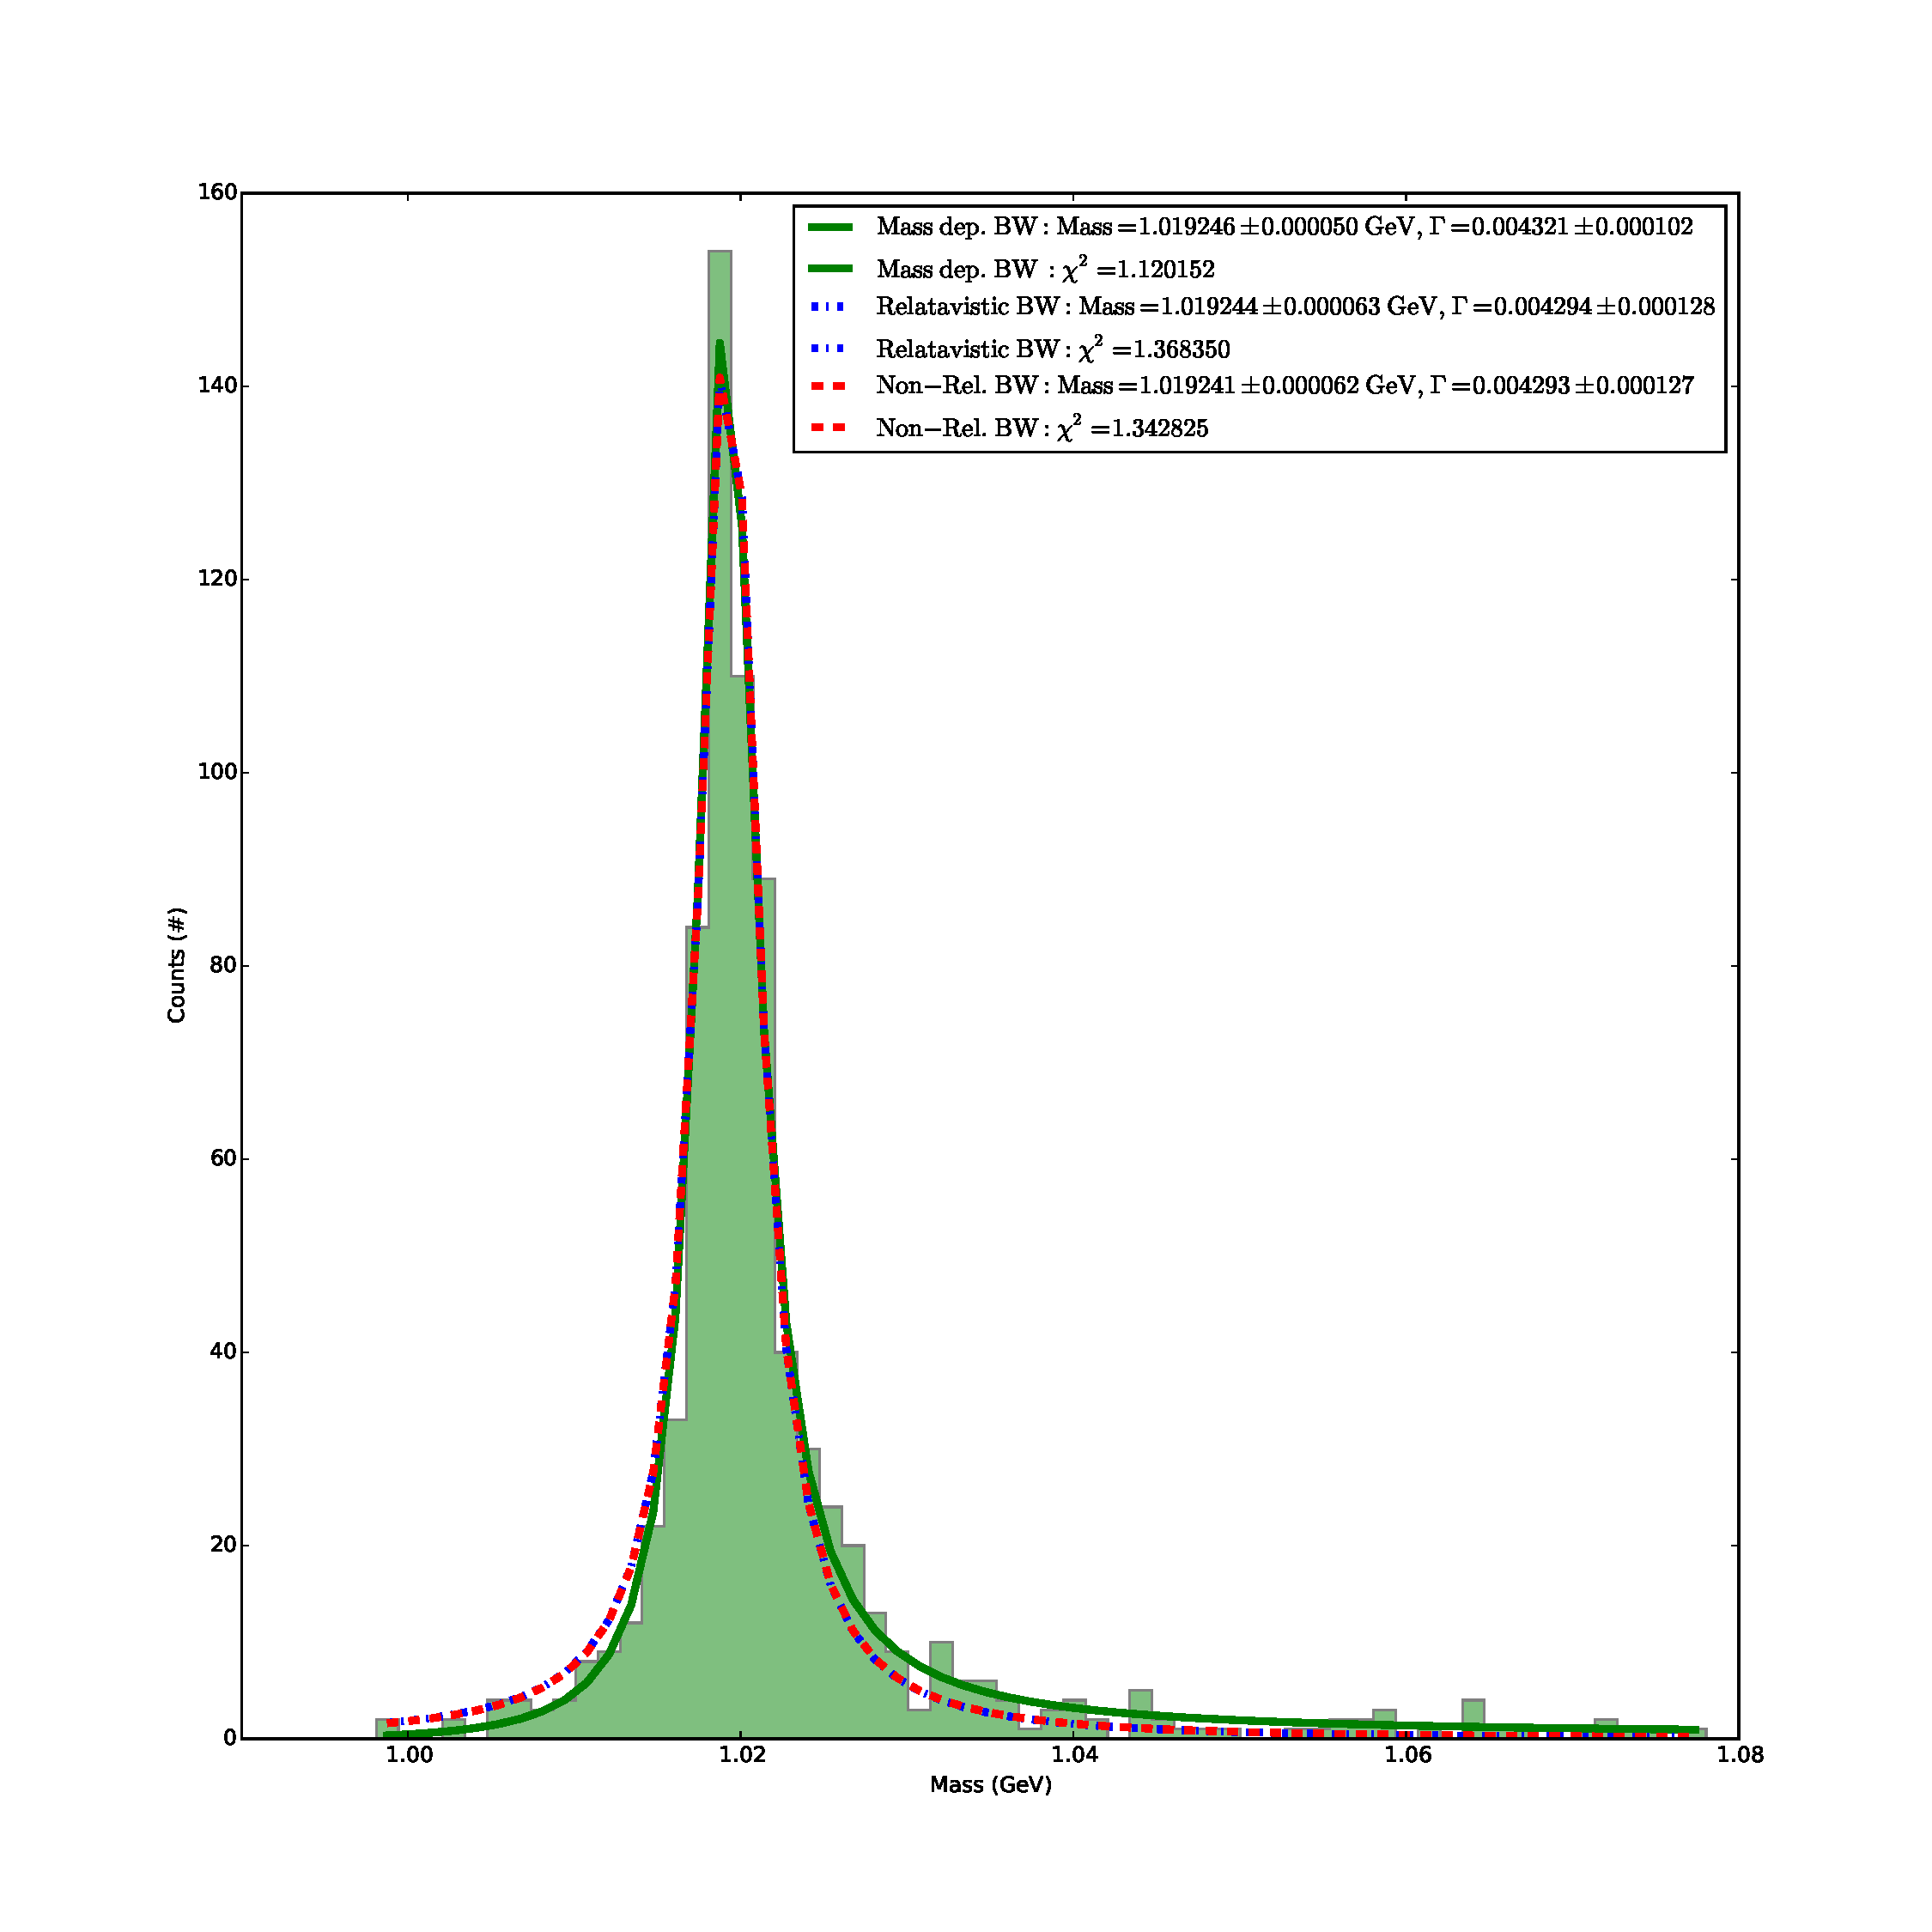
\includegraphics[scale=0.35]{Problem_1_and_2.pdf}\\
		\captionof{figure}{Three Breit-Wigner curves fit to data for, $\phi \rightarrow K^{+} K^{- }$}
		
	\pagebreak
	\item Stuff Here for problem 2.
	\item Stuff here for problem 3.
	\begin{center}
		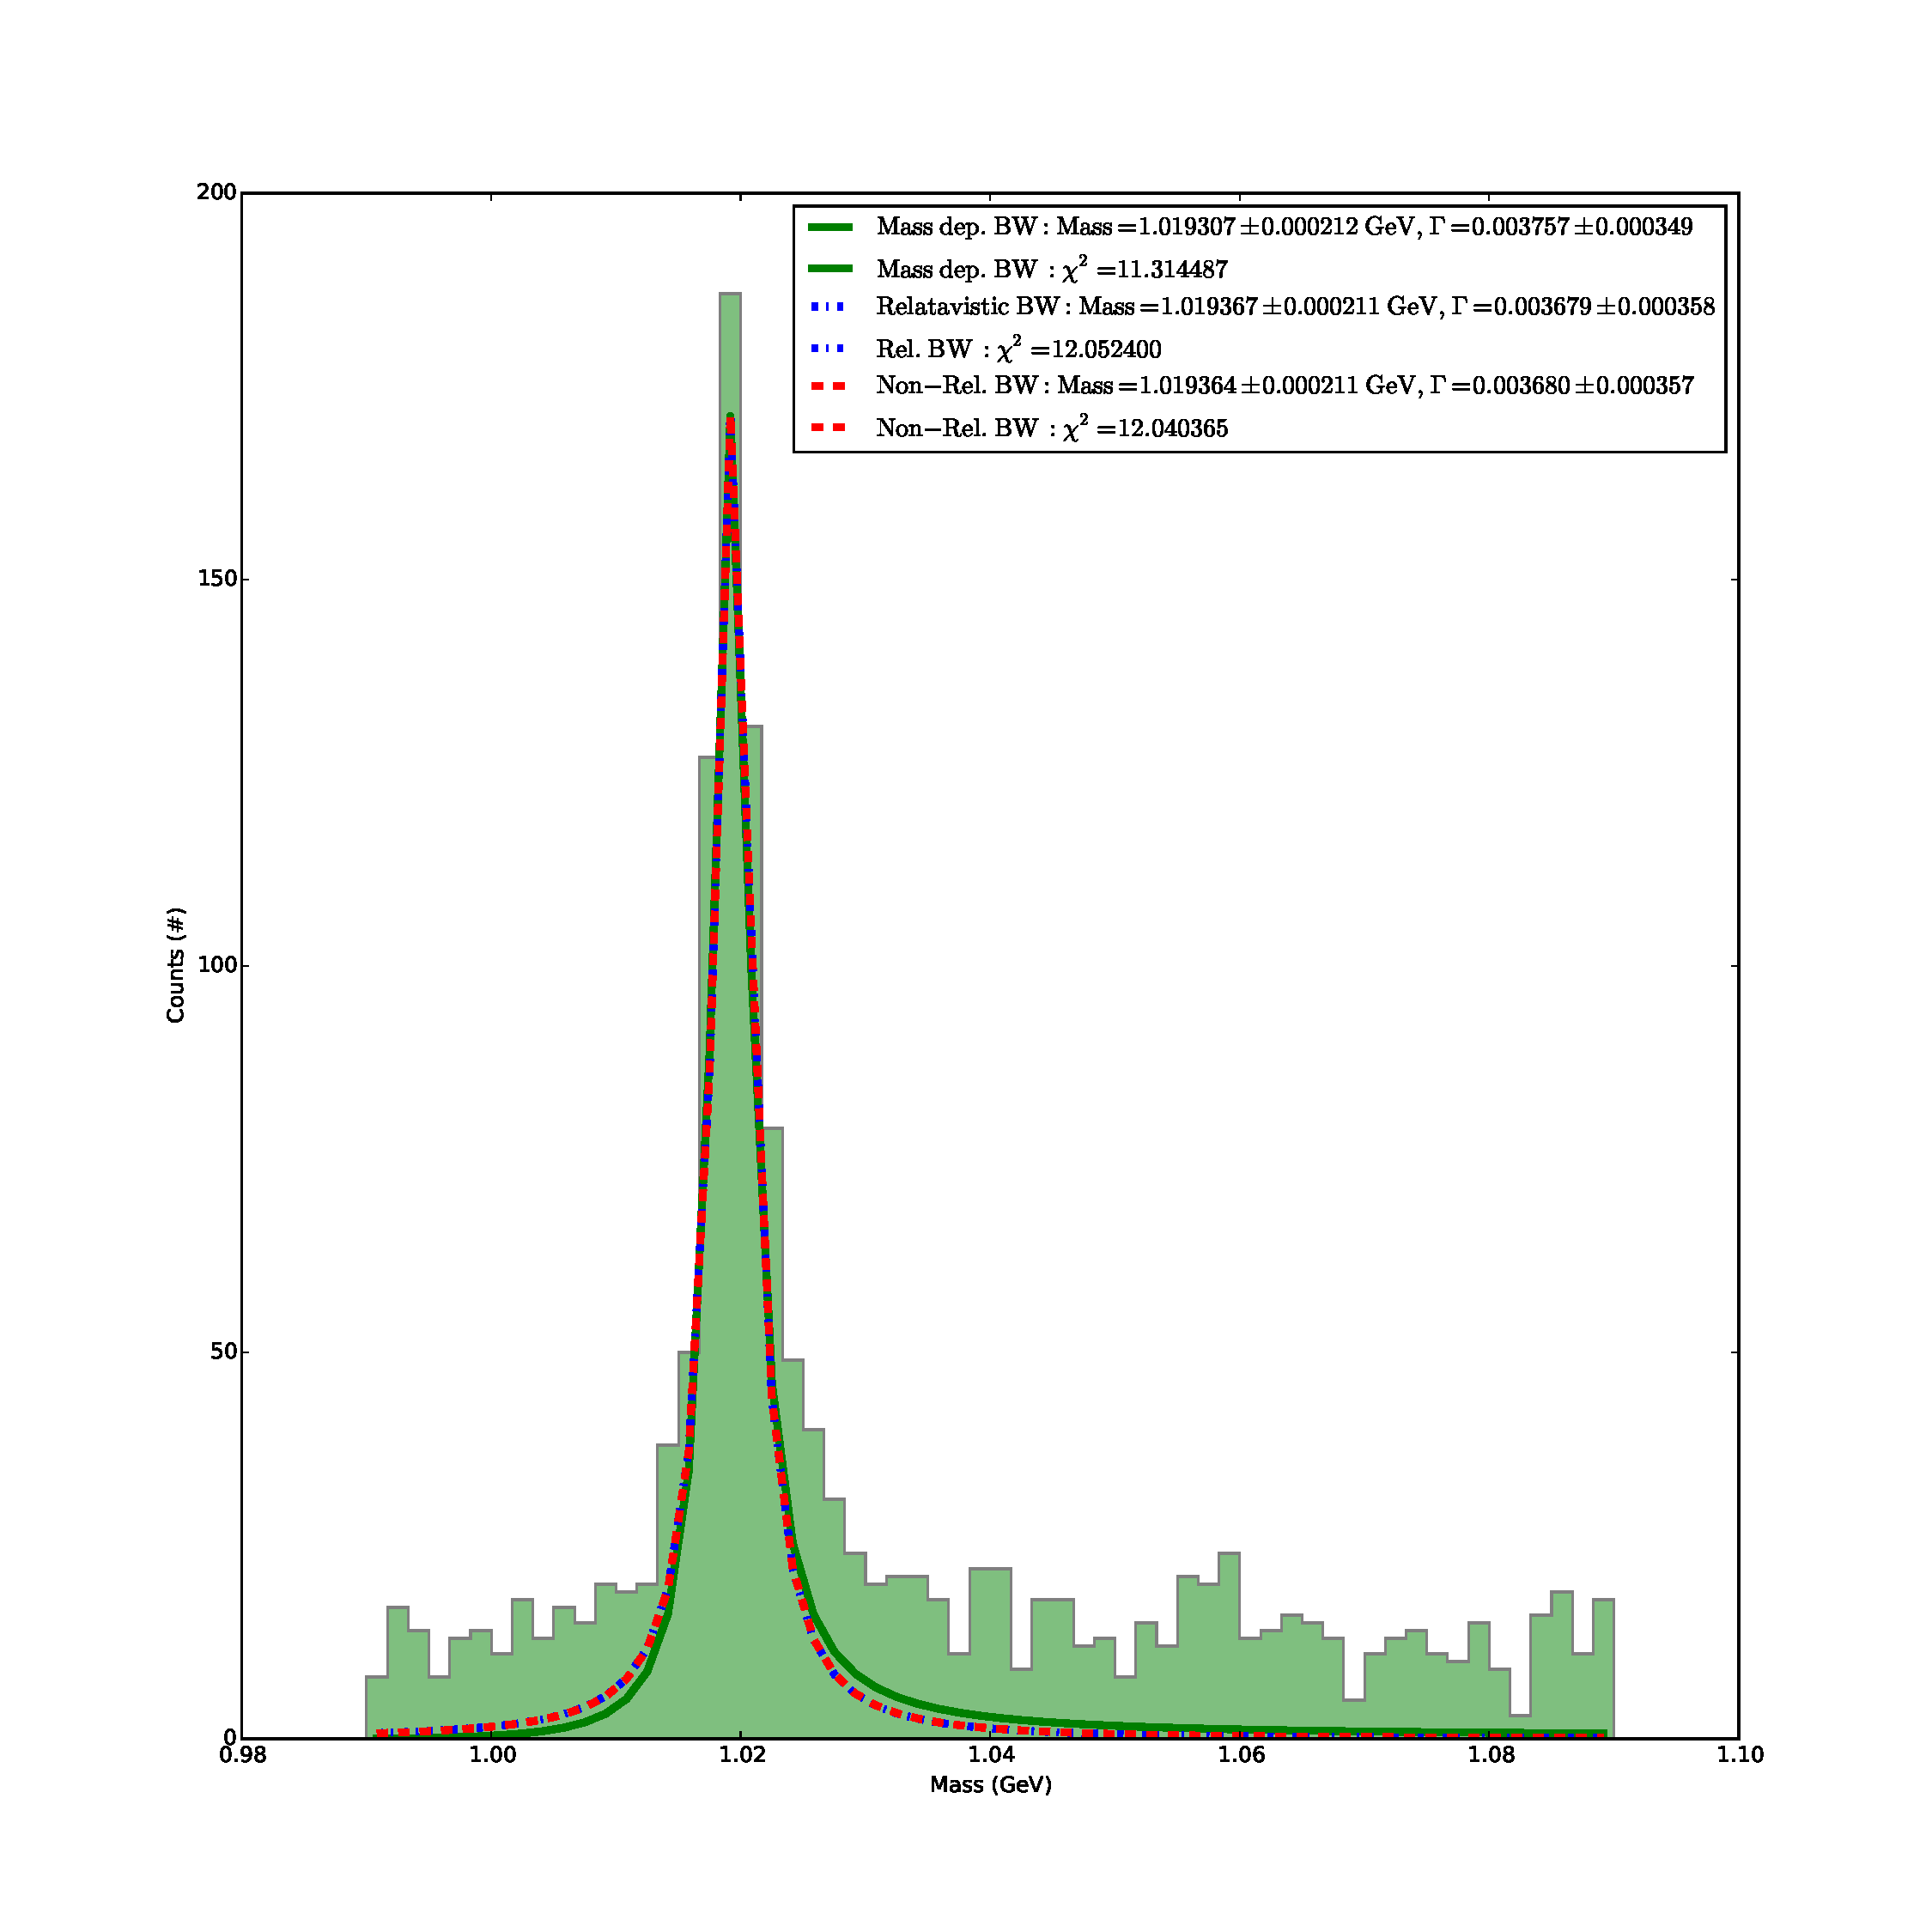
\includegraphics[scale=0.35]{Problem_3_nobackfit.pdf}
	\end{center}
		\captionof{figure}{Three Breit-Wigner curves with background fit to data for, $\phi \rightarrow K^{+} K^{- }$}
	\begin{center}
		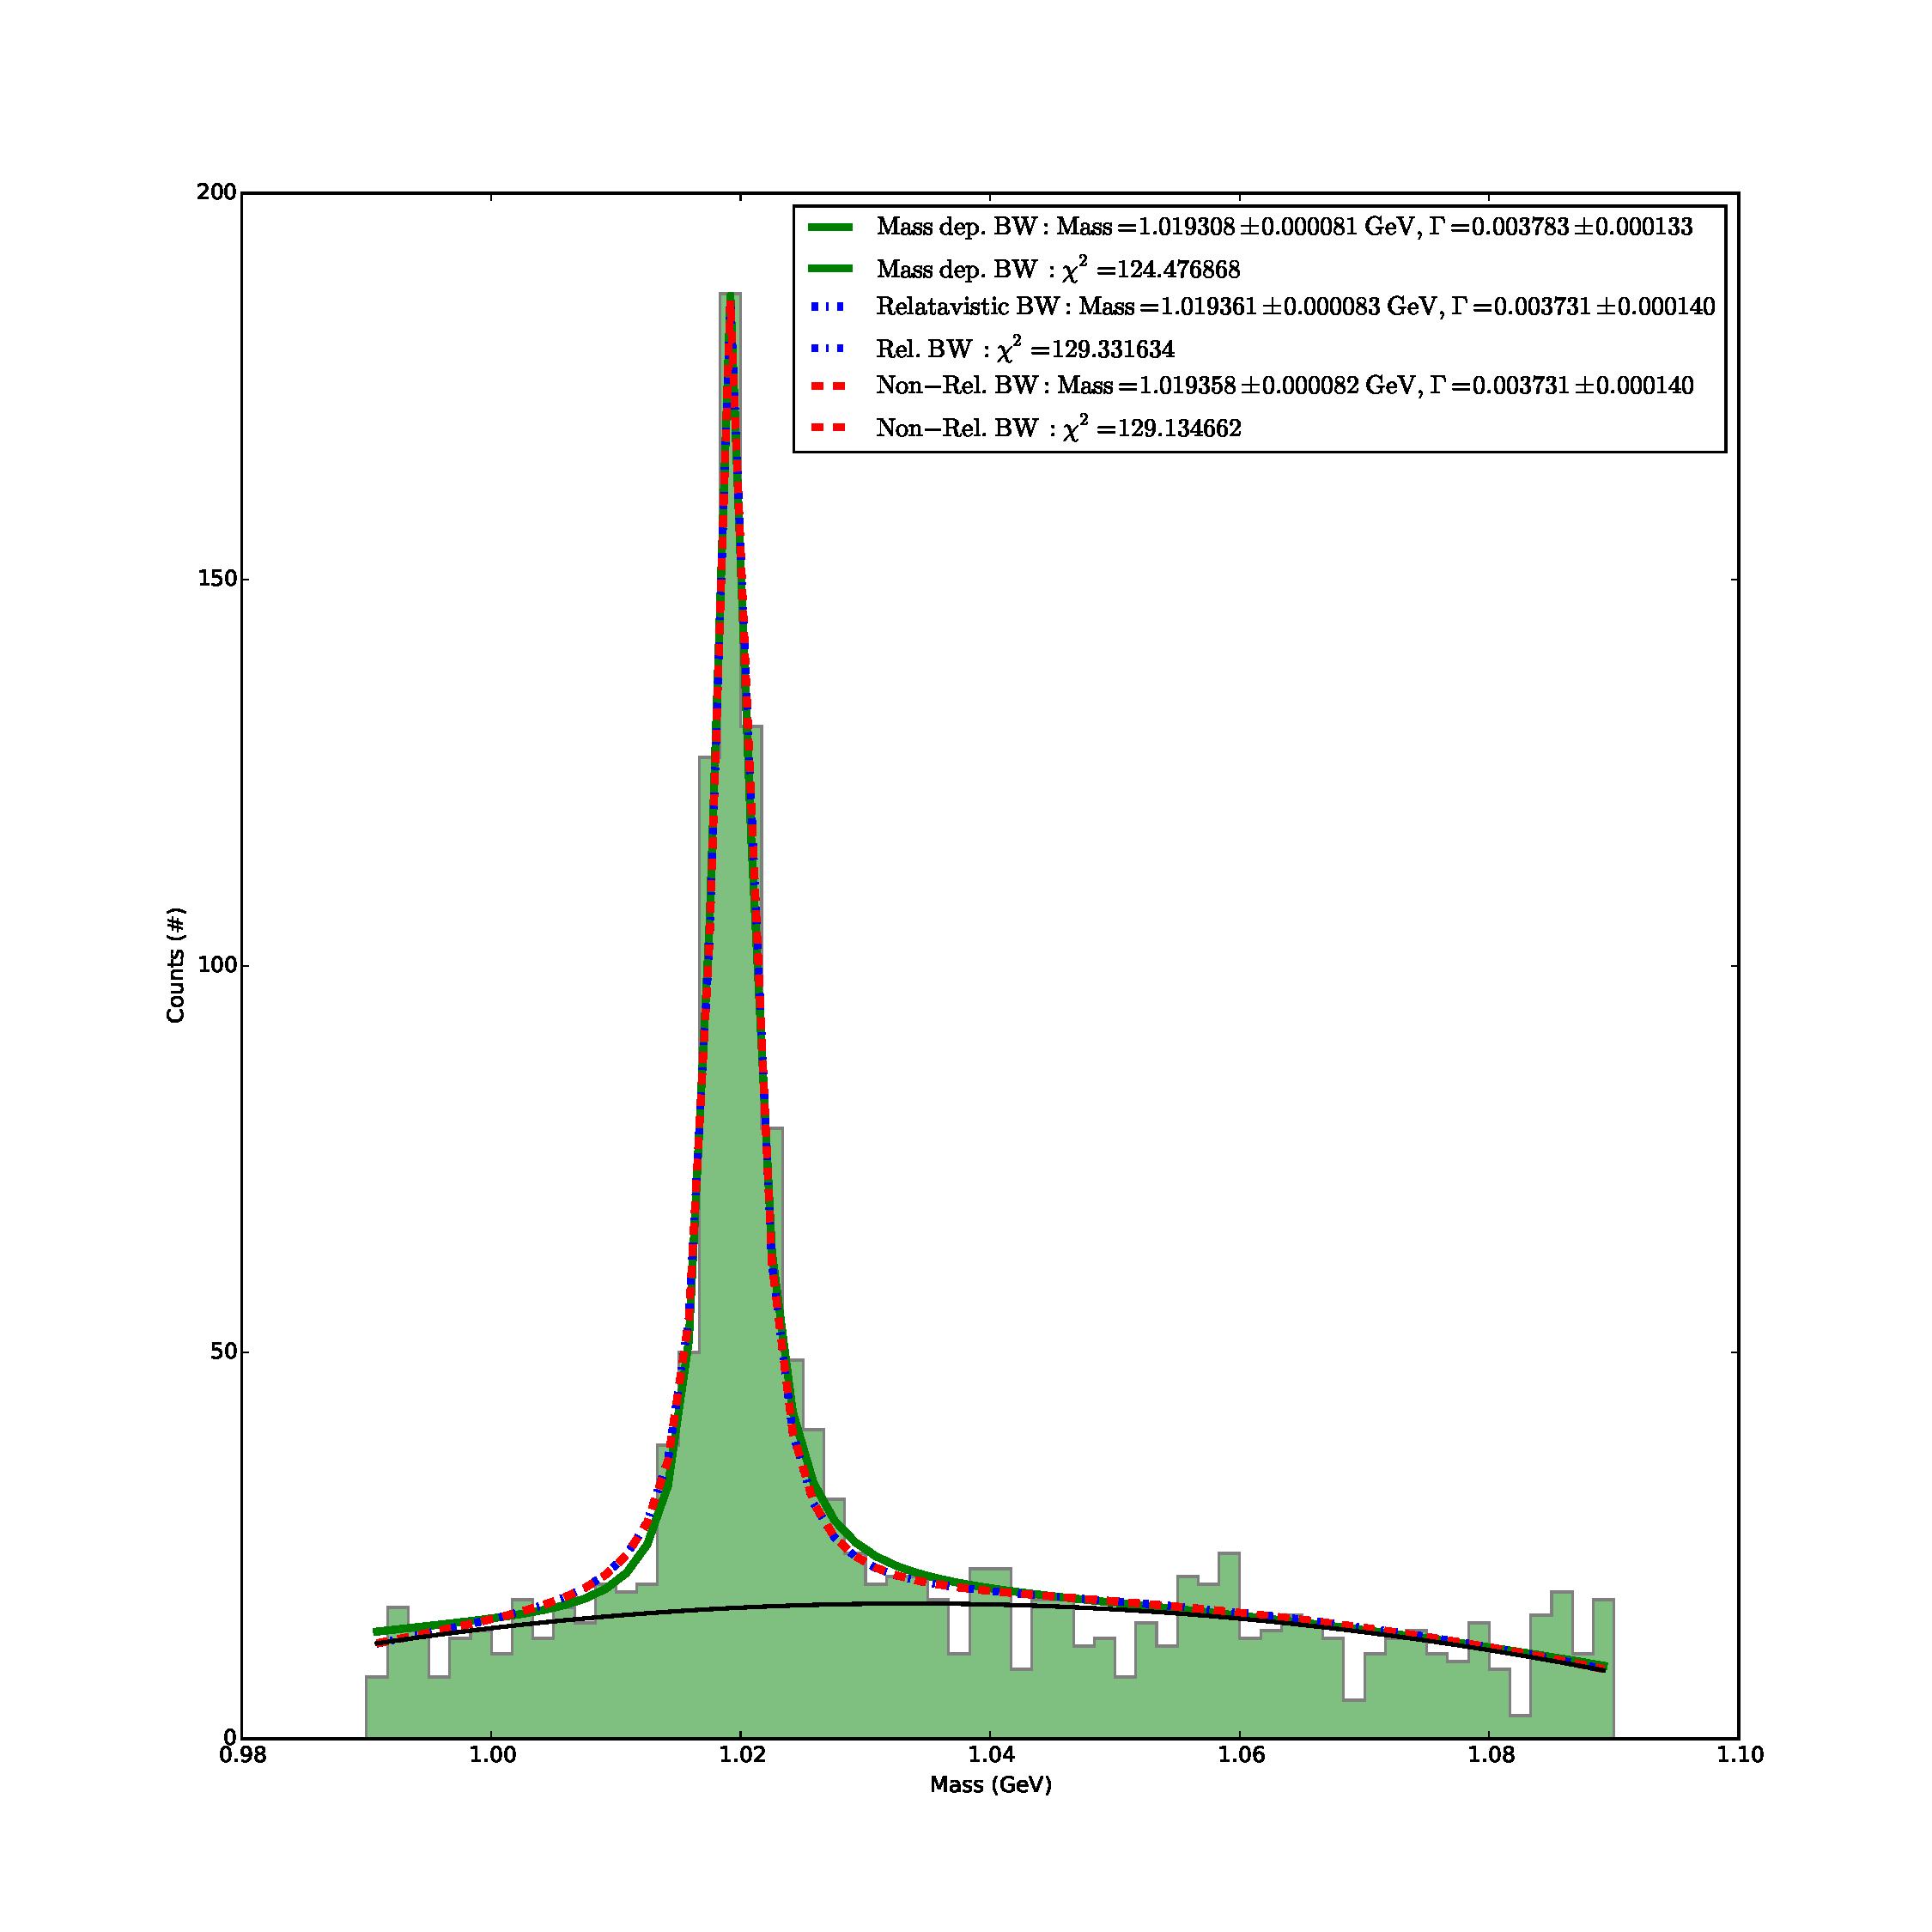
\includegraphics[scale=0.35]{Problem_3_withbackfit.pdf}
	\end{center}
		\captionof{figure}{Three Breit-Wigner curves with background fit with background for, $\phi \rightarrow K^{+} K^{- }$}

\end{enumerate}

\end{document}
